


\section{Geology of Migovec}

\subsection{The Julian Alps}
\label{sec:The Julian Alps}

\paragraph{Geography} 
\label{par:Geography} 
\passage{Tolminski Migovec} belong to the \passage{Julian Alps}, in the easternmost sector of the \passage{Southern Alps} \citep{bavec2004late}. 
They are bounded by the Pannonian and  Fruili-Venetian bassins to the east and west respectively, while to the north, they are separated from the Eastern Alps by the Periadriatic lineament \fref{map:geol large scale}. Beyond the South Alpine front, they become the Dinarides \citep{placer1998contribution,burrato2008sources}.
This carbonate dominated massif is characterised by high relief with valleys often 100-400m asl and high peaks reaching often above 2000m asl, and in the heart of the Triglav massif, the highest peaks are in excess of 2500m asl  \citep{vsmuc2009tectonic}. Relief production is attributed to both tectonic processes and glaciation, and \citet{vsmuc2009tectonic} argue for the primacy of the litho-sructural setting for the observed meso (1-10m) and macro- (100-1000m) scale relief.


\paragraph{Structural style}
\label{par:Structural style}
Overall, the tectono-stratigraphic setting \marginnote{The interplay between relief generation, erosion and sedimentary deposition during \emph{orogenesis} or moutain building events} of the \passage{Julian Alps} is a result of continued northward motion (about 2mm.a$^{-1}$ \citep{burrato2008sources} and since the Miocene,  counter-clockwise rotation of the Adriatic microplate \citep{marton2003palaeomagnetic}. 
The convergence of the Adria microplate with the Eurasian plate is quantitatively described by GPS velocity fields \citep{grenerczy2005tectonic}. 
Such convergence was led to the formation of Alpine and Dinaric mountain chains, and still generates earthquakes today ($M_w$ > 5) in the brittle deformation zone.

Slovenia, and in particular the area north east of Tolmin are located in the north-eastern corner of the Adria-Europe collisional belt. 
This area, at the critical juncture between the Alpine and Dinaric chains overlook rim of high topography around the relatively rigid, undeformed Adria microplate, which is only exposed in the Istria peninsula \citep{vsmuc2009tectonic}. 
It is buried under a thick cover of foredeep \marginnote{foredeep basins form in the immediate vicinity of collisional belt as thickened crust deforms the somewhat elastic plate underneath, creating a trough where the material sourced from the nearby mountains is preferentially deposited}sediments in the Friuli-Venetian plain. 

\paragraph{Alpine deformation}
\label{par:alpine deformation}



\paragraph{Present day stress regime}
\label{par:present day stress regime}
The activity on this heavily faulted boundary between Adria and Eurasia is highlighted by recent destructive earthquakes: Mw 6.4 on the Italian side in 1976 \citep{pondrelli2001seismotectonic}, and Mw 5.7 and Mw5. on the Slovenian side in 1998 \citep{bajc20011998} and 2004 \citep{aoudia2005july}. 
To highlight the vulnerability of this region, it is also worth keeping in mind that the largest earthquake ever at this junction b was the 1511 western Slovenia earthquake (M = 6.8). It is believed to have resulted in at least 12,000 deaths \citep{fitzko2005constraints}.
Fault plane solutions for the many Mw4-6 regional quakes demonstrate that the mode of deformation on the Italian side is chiefly by thrusting \citep{poli2002new}, while deformation is accommodated by dextral slip on the Slovenian side \citep{poljak2000seismotectonic}. 
The main strike-slip faults in NW Slovenia i.e. the Idrija, Ravne and Sava faults from south to north have a spectacular topographic expression. 

Indeed, the Ravne and Idrija faults' expression was mapped by \citet{cunningham2006application} with the aid of LiDAR data. The Ravne fault is \~35km long, yet seismic source modelling suggests a 13km only segment was involved in the 1998 earthquake, therefore it is possible that this fault generated stronger earthquakes in the past; it is thought it was involved in the devastating 1511 earthquake \citet{fitzko2005constraints}.
On the following geological map \fref{map:mapofgeology} the NW-SE trending fault passes to the NE of \passage{Krn}, between \passage{Gru\v{s}nica} and \passage{Tolminski Migovec} and heads towards \passage{Tolminske Ravne} hamlet.

Crucially, the Ravne fault segments pass through the \passage{Tolminka} springs basin, and its Quaternary (3Ma to Present) activity has played a primary role in the building local topography of the Tolminka valley (±1200m relief), which is described as a small pull-apart basin \citet{cunningham2006application}. 
In short this basin highlights the interplay between old Alpine structures, recent cross-cutting faults, glacial and hillslope erosional processes and karst development.

\paragraph{Conclusion}
\label{par:Conclusion}
As such, \citet{vsmuc2009tectonic} recognise four main landscape building events in the area of the Triglav lakes valley, located just 10km to the east of \passage{Tolminski Migovec}.

\begin{citemize}
\item The transport of the Mesozoic carbonate platforms which form the \passage{Julian Alps} as described by \citet{placer1998contribution}.
\item Miocene faults cross cutting 
\item Neogene strike-slip faulting cross-cutting the Alpine generated topography, producing youthful landforms \citep{vsmuc2009tectonic,cunningham2006application}
\item Karstic processes \citep{}
\end{citemize}
Overall they ascribe a tectonic topography to the area.

First 

\begin{map}[b!]
\checkoddpage \ifoddpage \forcerectofloat \else \forceversofloat \fi
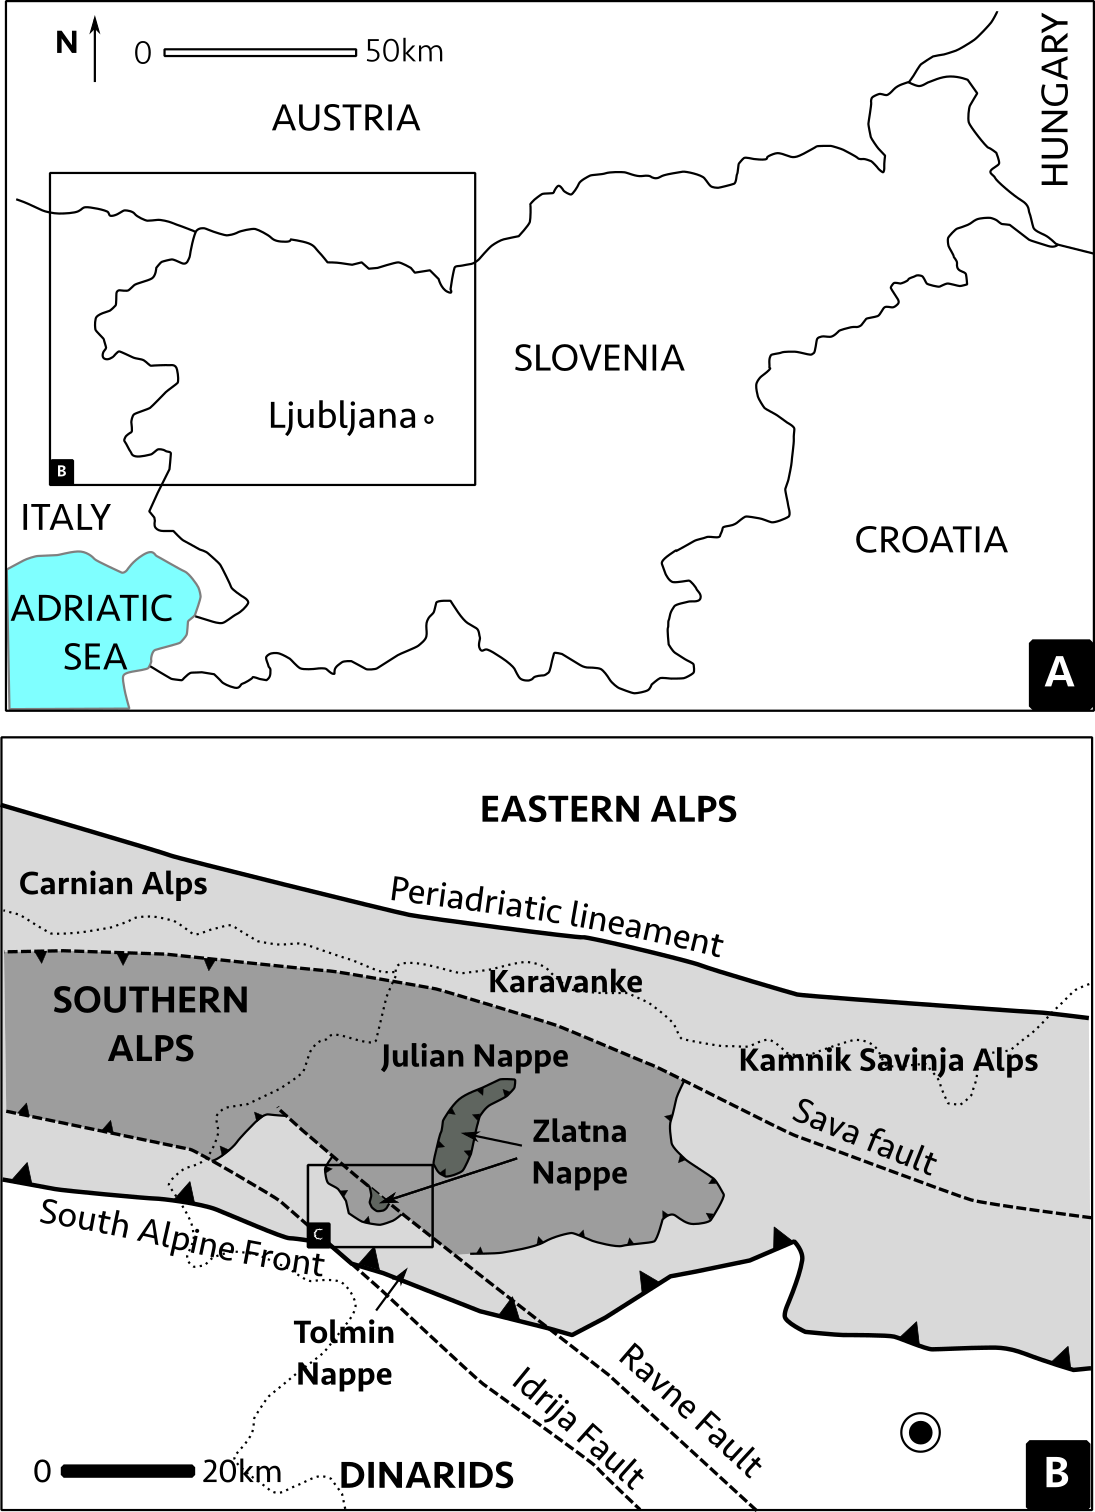
\includegraphics[width = \textwidth]{images/maps-of-mig/geology_large.png}
\caption[Structural setting of NW Slovenia]{The structural setting of northwestern Slovenia shows the \protect\passage{Tolmin} area straddling the active \protect\passage{Idrija} and \protect\passage{Ravne} faults. The \protect\passage{Migovec System} is developed within the Slatna overthrust and the underlying Dachtsein limestone, as shown in the geological map from \citet{buser1986tolmavc}. Figure modified from \citet{vsmuc2009tectonic}}
\label{map:geol large scale}
\end{map}

\subsection{Tolminski Migovec}
\emph{Lithology is a summary of the gross characteristics of the rock.}

\fref{map:mapofgeology}
\passage{Tolminski Migovec} is mainly formed by a sequence of massive to well-bedded (1-3m) pure grey to buff limestones with patches of dolomite \citep{buser1986tolmavc}. Most of the mountain bedrock was formed during the Upper Triassic Norian to Rhaetian age (228 -101.3 Ma) and represents a large carbonate platform located in the NW corner of the Tethys palaeo-ocean. This formation, which goes under the name of `\passage{Dachstein}' limestone (in Slovene 'Dachteinski apnenec', is a key member of both the \passage[Calcareous Alps]{Southern Calcareous Alps} and \passage{Northern Calcareous Alps}. Debate is ongoing as to the origin of the cyclic pattern of the limestone beds called Lofer cyclothems (sequences tracking a shallowing-up depositional environment), with some authors favouring local tectonic control over orbitally forced sea-level changes (see Milankovitch cycles\sidenote{These cycles are related to \emph{precession}, \emph{tilt} and \emph{ellipticity}}).


\margininbox{On limestones}{Calcium Carbonate --- $CaCO_3$ ---  dominates the mineralogy of limestones, which can be identified with a simple hydrochloric acid test. The death and accumulation of carbonate secreting organisms is the main process by which a calcite dominated sedimentary rock forms, and the distinct fossil assemblages preserved in the rock record serves to date the formations and attach them to an environment of deposition. The long subsequent geological history of uplift, deformation --- a pressure-temperature path through time --- are partially recorded, superimposed as microscopic fabrics, mineral replacement, macroscopic folding or faulting.}{\logbook}

 \begin{pagemap}
 \checkoddpage \ifoddpage \forcerectofloat \else \forceversofloat \fi
\centering
  \includegraphics[width=\textwidth]{"images/maps-of-mig/geological_map_with_symbols".png}
  
  \caption{Geological map of the Tolmin Area, extracted from \textit{Buser, et al, 1987 Tolmin in Videm, Carta Geologica 1:100 000, Ljubljana} and projected on the Slovenian National Grid ESPG 3794}
  \label{map:mapofgeology}
 \end{pagemap}

\subsection{Structural setting}
\emph{The structural setting refers to the past and present tectonic stresses in a given area, and how these were accomodated through folding and faulting.}

The carbonate succession was then transported to the SW as part of the Slatna thrust complex and overlie younger Jurassic and Cretaceous formations exposed further down the valley. The \passage{Tolminski Migovec} cavernous limestones are overall gently folded in a WSW dipping syncline, with parasitic (smaller wavelength) folds and offsetting faults with displacement of 1-3m.

 The NNW-SSE oriented mountain ranges belong to the \passage{Julian Alps}, one of the most southerly massifs of the European Alps and occupy a critical place at the juncture between the Alpine and Dinaride chains. 
 
 
\begin{marginfigure}
\checkoddpage \ifoddpage \forcerectofloat \else \forceversofloat \fi
\centering
 \frame{\includegraphics[width=\linewidth]{"images/maps-of-mig/marls_limestone".jpg}} 
 \caption{An example of the Jurassic marl and limestone succession, with pyrite nodules and minor fault offsetting the thick micritic limestone beds \pic{Tanguy Racine} on the \protect\passage{Slovenska Geolo\v{s}ka Pot}}
 \label{marls and limestones}
\end{marginfigure}

 The block is bounded to the South West by a major strike slip fault, the Ravne fault, active as recently as April 1998 when an earthquake of magnitude 5.5 on the Richter scale struck near Tolminski Migovec.

Since their emergence as part of the Alpine chain, the carbonate sediments were subjected to two distinct erosional regimes. In recent glacial periods, glaciers originating from high cirques carved over-steepened or U-shaped valleys, plucking, crushing and carrying large amounts of sediments. Both the valleys and sediments preserved on their sides are an archive of past glacial events: direction of ice flow, duration and intensity of the period. Second the dissolution of carbonates in the presence of weakly acidic rain sculpted a karstic landscape; karstic landforms, such as underground drainage only develop if dissolution is the principal agent of erosion. Otherwise, physical processes, such as hillslope stabilisation, tend to obscure the weaker effect of dissolution by mechanical failure of the rock.
